% ==============================================================================
% EE413A
% Lab 1 - Transistors and Amplifiers
% ---------------------------------
% Last updated 2015-01-12-
%
% Author:
% Jonas Sjöberg     <tel12jsg@student.hig.se>
% Esther Hedlund    <tfk13ehd@student.hig.se> 
%
% License:
% Creative Commons Attribution-NonCommercial-ShareAlike 4.0 International
% See LICENSE.md for full licensing information.
% ==============================================================================


% ==============================================================================
% INCLUDES AND CONFIGURATION
% ==============================================================================
\documentclass[11pt,a4paper]{article}

\usepackage[T1]{fontenc}
\usepackage{lmodern}
\usepackage[utf8]{inputenc}
\usepackage{siunitx} % Provides the \SI{}{} and \si{} command for typesetting SI
\usepackage{amssymb}
\usepackage{amsmath}
\usepackage{amsfonts}
\usepackage{graphicx}
\usepackage{longtable,booktabs}
\usepackage{microtype}
\usepackage[hidelinks]{hyperref}

\setlength\parindent{0pt} % Removes all indentation from paragraphs

% ==============================================================================
% DOCUMENT METADATA 
% ==============================================================================
\title{EE413 \\ Lab 138 \\ Transistors and Amplifiers}
%\author{{Jonas Sjöberg} \and {Esther Hedlund}}

\author{\\
  Jonas Sjöberg\\
  Högskolan i Gävle,\\
  Elektronikingenjörsprogrammet,\\
  \texttt{tel12jsg@student.hig.se}\\
  \\
  Esther Hedlund\\
  Högskolan i Gävle,\\
  Elektronikingenjörsprogrammet,\\
  \texttt{tfk13ehd@student.hig.se}\\}

\date{}
% ==============================================================================
\begin{document}
% ==============================================================================
\maketitle

\begin{center}
\begin{tabular}{l r}
    Data Performed: & 26 November 2014 \\
    Instructor: & Nauman Masud, Shoaib Amin
\end{tabular}
\end{center}

% ==============================================================================
% ABSTRACT
% ==============================================================================
\begin{abstract}
This lab is meant to teach and show the practical use of bipolar junction transistor amplifiers. The lab includes constructing and measuring DC circuits, calculating biasing networks, amplification, bandwidth and plotting characteristic curves of circuit parameters.
\end{abstract}

\newpage

% ==============================================================================
% TABLE OF CONTENTS
% ==============================================================================
{
\hypersetup{ 
	colorlinks=true,
	citecolor=black,
	filecolor=black,
	linkcolor=black,
	urlcolor=black
}
\setcounter{tocdepth}{3}
\tableofcontents
}

\newpage

% ==============================================================================
% SECTION: Ic-Uce-characteristics
% ==============================================================================
\section{Ic-Uce-characteristics}\label{ic-uce-characteristics}

\subsection{Circuit}\label{circuit}
% ------------------------------------------------------------------------------

\begin{figure}[htbp]
    \centering
    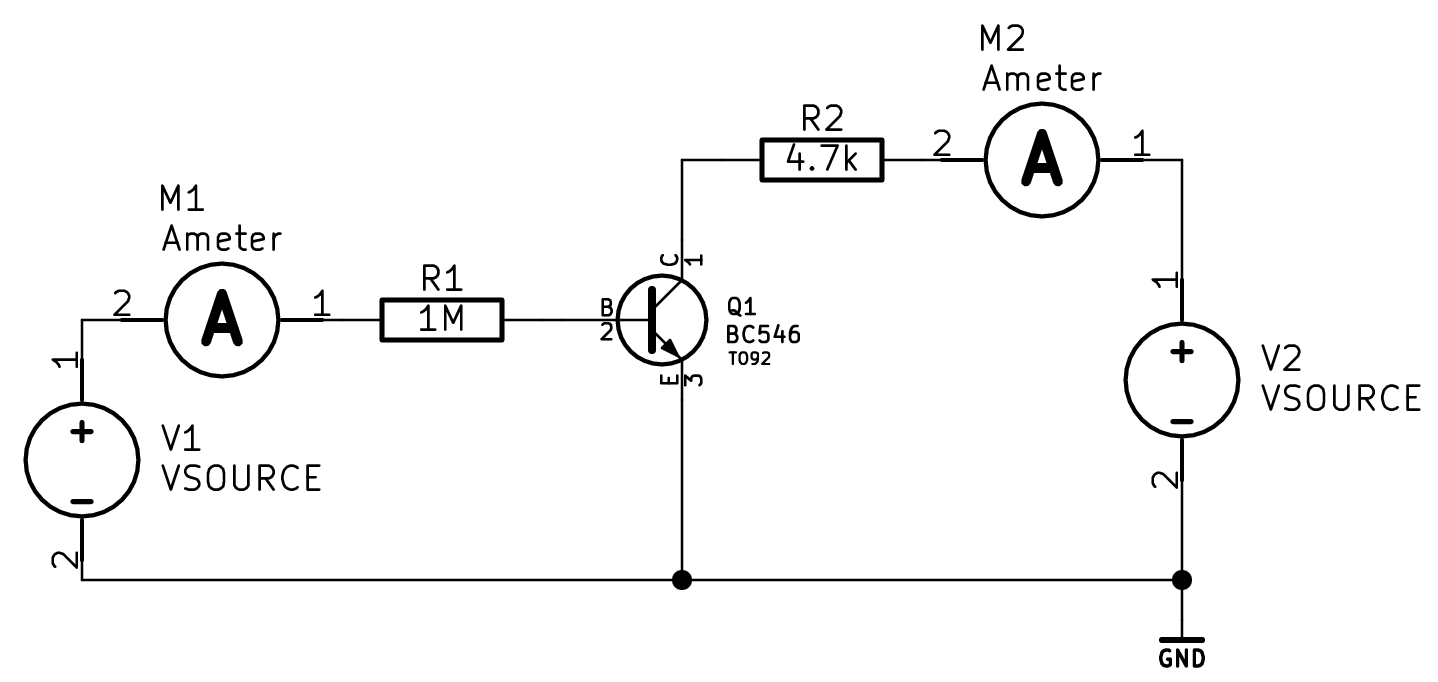
\includegraphics[width=0.75\textwidth]{img/ic-uce_schem}
    \caption{Measurement setup schematic}
    \label{fig:ic-uce_schem}
\end{figure}

\subsection{Fixed collector voltage}\label{fixed-collector-voltage}
% ------------------------------------------------------------------------------

With the collector resistor $R_{2}$ left out or shorted, an adjustable power
supply is connected directly across the collector-emitter junction,
fixing the collector voltage. First we get the base currents for known
collector currents. Adjusting voltage $V_{1}$ translates to varying the base
current $I_{b}$ and in turn the collector current $I_{c}$. The transistor used is
a BC547C.

\subsection{Measurements}\label{measurements}
% ------------------------------------------------------------------------------

\begin{longtable}[c]{@{}l@{}l}
\toprule\addlinespace
$I_{c}$ (mA) & $I_{b}$ ($\mu$A)
\\\addlinespace
\midrule\endhead
0.5 & 1.14
\\\addlinespace
1.0 & 2.11
\\\addlinespace
1.8 & 3.72
\\\addlinespace
\bottomrule
\addlinespace
\caption{Measurement of $I_{b}$ and $I_{c}$}
\label{ic_ib}
\end{longtable}

The base current is then held at a constant value and the
collector-emitter voltage is swept over a range of 0-10V in 1V steps.
The results is given in Figure~\ref{fig:ic-uce_plot}.

\begin{figure}[htbp]
    \centering
    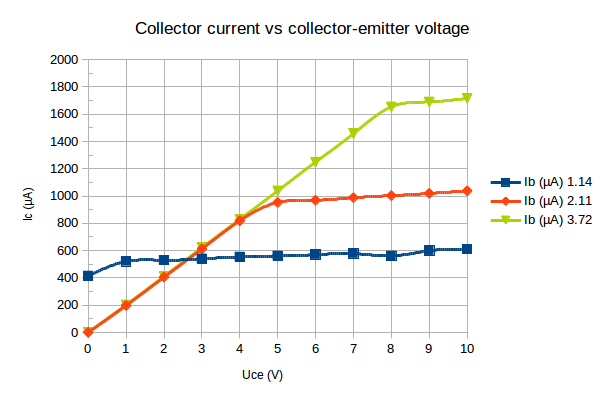
\includegraphics[width=\textwidth]{img/ic-uce_plot}
    \caption{$I_{c}$ as a function of $V_{ce}$}
    \label{fig:ic-uce_plot}
\end{figure}

\subsection{Simulation}\label{simulation}
% ------------------------------------------------------------------------------

Spice circuit simulation with the setup shown in Figure~\ref{fig:ic-uce_ltspice-schem}
confirms that measurements reflect typical bjt characteristics, shown in 
Figure~\ref{fig:ic-uce_ltspice-plot}.
The program used is Linear Technology LTspice, with a transistor model based on transistor datasheet values.


\begin{figure}[htbp]
    \centering
    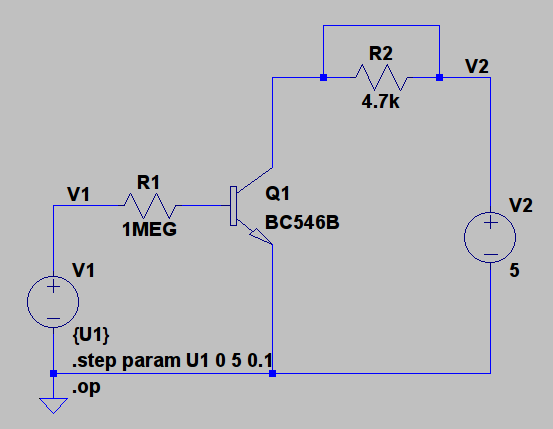
\includegraphics[width=0.75\textwidth]{img/ic-uce_ltspice-schem.png}
    \caption{Simulation setup measuring $I_{c} / V_{ce}$}	% Ic/Uce
    \label{fig:ic-uce_ltspice-schem}
\end{figure}

\begin{figure}[htbp]
    \centering
    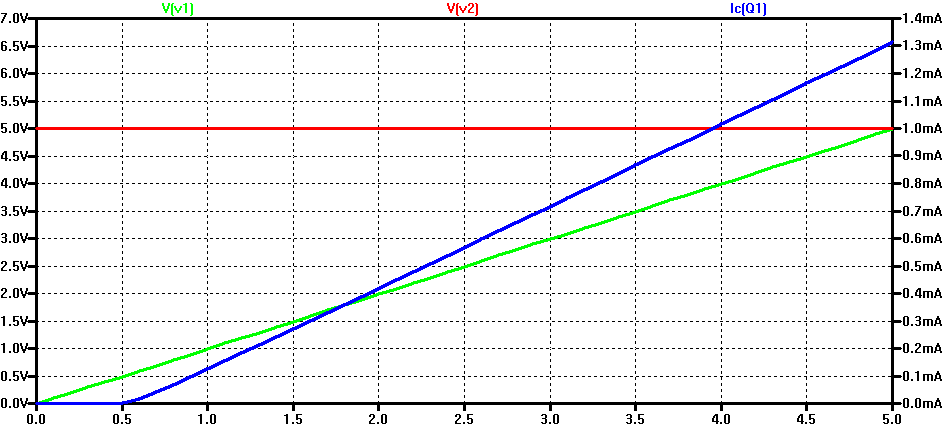
\includegraphics[width=\textwidth]{img/ic-uce_ltspice-plot.png}
    \caption{$I_{c} / V_{ce}$ simulation plot}
    \label{fig:ic-uce_ltspice-plot}
\end{figure}


% ==============================================================================
% SECTION: Quiescent conditions
% ==============================================================================
\section{Quiescent conditions}\label{quiescent-conditions}
The calculated results for the basic circuit is shown in Figure~\ref{fig:load-line_plot}.

\begin{figure}[htbp]
    \centering
    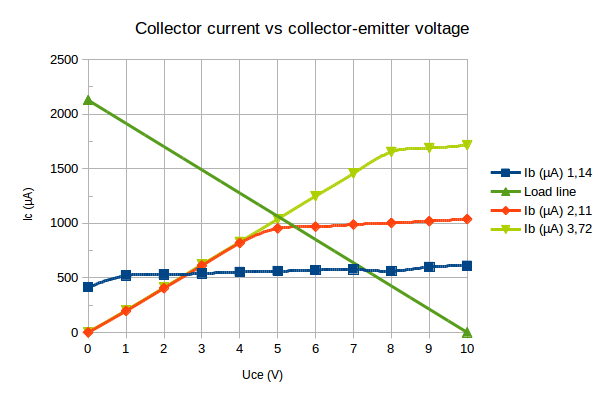
\includegraphics[width=\textwidth]{img/load-line_plot}
    \caption{Calculated load line.}
    \label{fig:load-line_plot}
\end{figure}

% ==============================================================================
% SECTION: Ib transfer function
% ==============================================================================
\section{Uce/Ib transfer function}\label{uceib-transfer-function}

Examine the output signal of the first circuit. Determine the linearity
of the output, as in the relation of $U_{ce}$ to $I_{b}$. Uses the measurement
setup and circuit shown in Figure~\ref{fig:ic-uce_schem}. The input voltage source is low
enough impedance to be considered constant. The linear region is very
small, the transistor is best used as a switch in this configuration.

\begin{figure}[htbp]
    \centering
    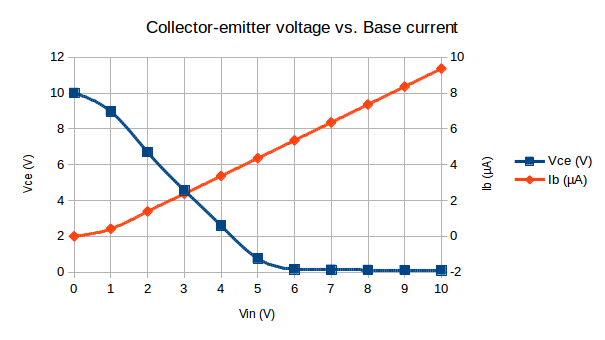
\includegraphics[width=\textwidth]{img/uce-ib_plot}
    \caption{$V_{ce}$ and $I_{b}$ as a function of input voltage.}
    \label{fig:uce-ib_plot}
\end{figure}

% ==============================================================================
% SECTION: Ic/Ib characteristics and current amplification
% ==============================================================================
\section{Ic/Ib characteristics and current
amplification}\label{icib-characteristics-and-current-amplification}

\subsection{Measurements}\label{measurements-1}
% ------------------------------------------------------------------------------

Results for collector current as a function of base current is shown in Figure~\ref{fig:ic-ib_plot}.

The current gain, $\beta = \frac{I_{c}}{I_{b}}$ is shown in Figure~\ref{fig:ic-ib-amplification_plot}
as a function of base current, results in multiples and dBs.

\begin{figure}[htbp]
    \centering
    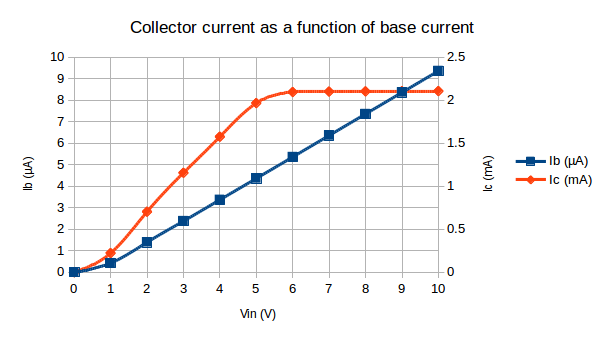
\includegraphics[width=\textwidth]{img/ic-ib_plot.png}
    \caption{$I_{c}$ as a function of $I_{b}$.}
    \label{fig:ic-ib_plot}
\end{figure}

\begin{figure}[htbp]
    \centering
    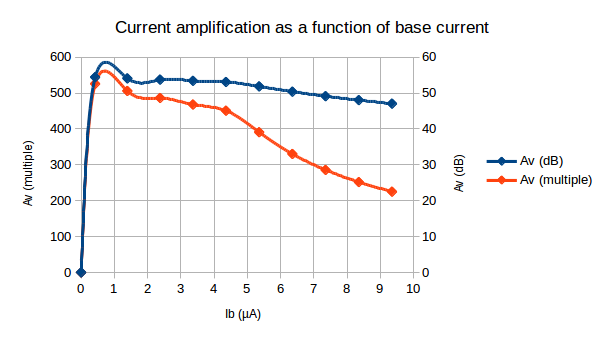
\includegraphics[width=\textwidth]{img/ic-ib-amplification_plot.png}
    \caption{Current gain, $\beta$ as a function of $I_{b}$.}
    \label{fig:ic-ib-amplification_plot}
\end{figure}


\subsection{Comments}\label{comments}
% ------------------------------------------------------------------------------

Current gain decreases with base current. This is one of many non-ideal
characteristics of the transistor. The phenomena is called a ``high
injection effect''. Source included in references.


% ==============================================================================
% SECTION: BJT biasing
% ==============================================================================
\section{BJT biasing}\label{bjt-biasing}

\subsection{Measurements}\label{bjt-biasing-measurements}
% ------------------------------------------------------------------------------
Making $V_{ce}$ 10V maximizes the dynamic range of the amplifier, I.E. improves
linearity and reduces clipping of higher amplitude signals, by centering the
operating "bias" point. The available voltage is split evenly between the three
droppers; collector resistor collector-emitter resistance and emitter resistor.
The circuit used is shown in Figure~\ref{fig:bjt-bias_1}.

\begin{longtable}[c]{@{}llll@{}}
\toprule\addlinespace
$R_{b}  (\Omega)$ & $V_{e}$ (V) & $R_{c}  (\Omega)$
\\\addlinespace
\midrule\endhead
390k & 10.3 & 1
\\\addlinespace
470k & 9.3 & 47
\\\addlinespace
560k & 8.2 & 1k
\\\addlinespace
680k & 7.7 & 1k
\\\addlinespace
820k & 6.8 & 1.2k
\\\addlinespace
1M & 5.9 & 3.3k
\\\addlinespace
\bottomrule
\addlinespace
\caption{Bias resistor with bias voltages}
\end{longtable}

\begin{figure}[htbp]
    \centering
    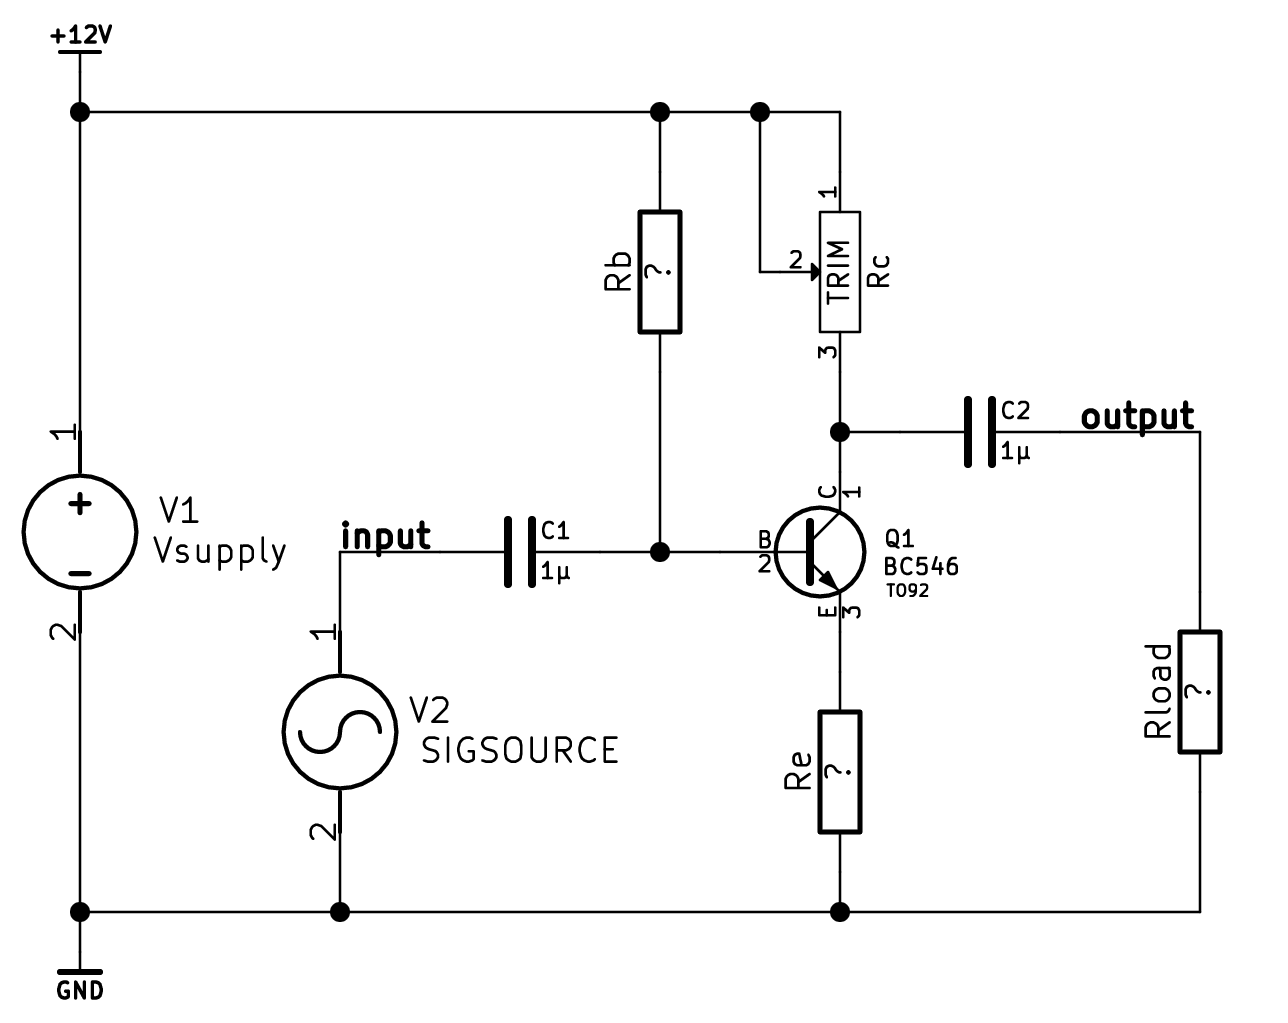
\includegraphics[width=0.75\textwidth]{img/bjt-bias_1.png}
    \caption{BJT biasing circuit, emitter impedance resistive.}
    \label{fig:bjt-bias_1}
\end{figure}

\subsection{Comments}\label{comments}
% ------------------------------------------------------------------------------
The collector resistor would have to be a short to put Vce at 10V. 
We come to the conclusion that this method of biasing is thoroughly unpractical.


% ==============================================================================
% SECTION: BJT amplifier
% ==============================================================================
\section{BJT amplifier}\label{bjt-amplifier}

\subsection{Measurements}\label{bjt-measurements}
% ------------------------------------------------------------------------------
An oscilloscope is used for measuring the amplifier gain with a 1kHz 1V peak to
peak sine wave. The circuit used is shown in Figure~\ref{fig:bjt-bias_1}, 
coupling is DC only. For the second measurement, a 100$\mu$F capacitor was connected
across the emitter resistor, the circuit is shown in Figure~\ref{fig:bjt-bias_2AC}.

\begin{figure}[htbp]
    \centering
    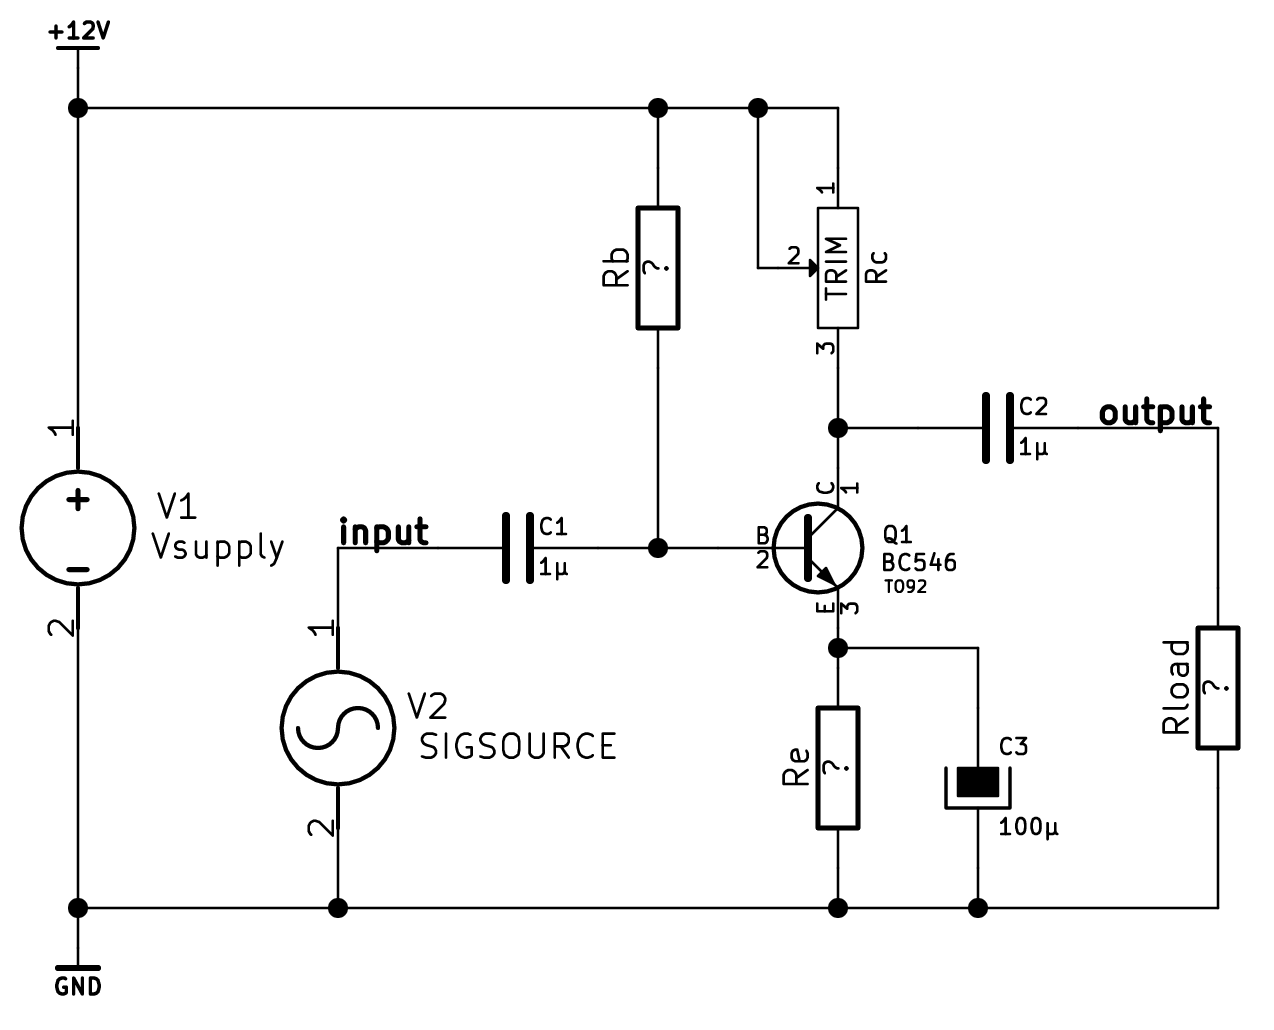
\includegraphics[width=0.75\textwidth]{img/bjt-bias_2AC.png}
    \caption{BJT biasing circuit, emitter AC bypassed.}
    \label{fig:bjt-bias_2AC}
\end{figure}

\subsubsection{Amplifier gain}\label{amplifier-gain}
% ------------------------------------------------------------------------------
%\begin{longtable}[c]{@{}lll@{}}
\begin{longtable}[c]{lll}
\toprule\addlinespace
Coupling & DC & AC
\\\addlinespace
\midrule\endhead
Input voltage ($mV_{pp}$) & 100 & 100
\\\addlinespace
Output voltage ($V_{pp}$) & 0.283 & 9.23
\\\addlinespace
Voltage gain (multiple) & 2.83 & 91.3
\\\addlinespace
Voltage gain (dB) & 9.04 & 39.2
\\\addlinespace
Phase shift (degrees) & 180 & 150
\\\addlinespace
\bottomrule
\addlinespace
\caption{Amplifier gain measurements}
\end{longtable}

\subsubsection{Frequency response}\label{frequency-response}
% ------------------------------------------------------------------------------
Measurement results for the circuit in Figure~\ref{fig:6_amplifier-av_schem} are shown in Figure~\ref{fig:6_amplifier-av_bode}.
Frequency response shows no high frequency rolloff in the audible frequency
range 20Hz-20kHz. There is however a high frequency limit, set primarily by
stray capacitances in breadboards and such.

\begin{figure}[htbp]
    \centering
    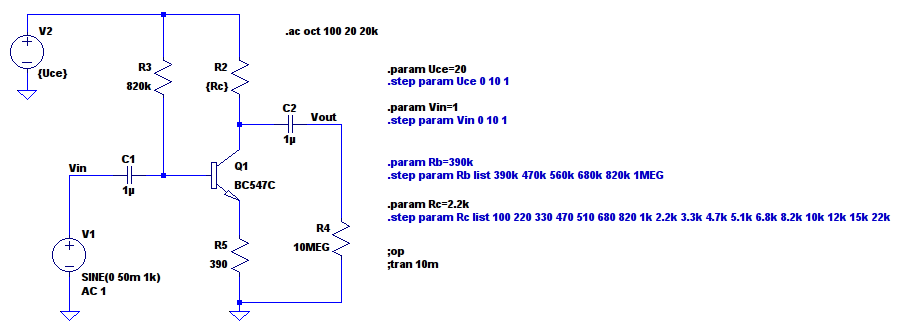
\includegraphics[width=\textwidth]{img/6_amplifier-av_schem.png}
    \caption{Amplifier frequency response circuit.}
    \label{fig:6_amplifier-av_schem}
\end{figure}

\begin{figure}[htbp]
    \centering
    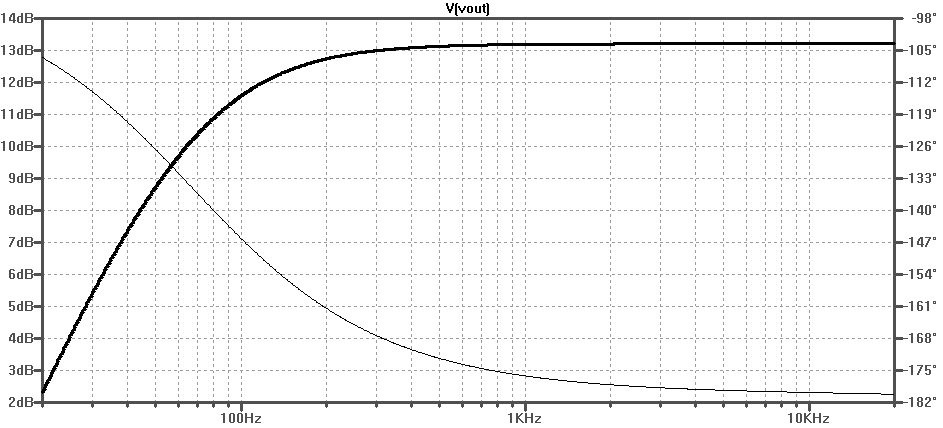
\includegraphics[width=\textwidth]{img/6_amplifier-av_bode.png}
    \caption{Amplifier frequency response and phase shift.}
    \label{fig:6_amplifier-av_bode}
\end{figure}


\subsection{Improved biasing}\label{improved-biasing}
% ------------------------------------------------------------------------------
The one resistor base bias is in practice not very reliable as it is dependant
on transistor beta. A more practical design that scales better for production
adds a second resistor, forming a voltage divider that fixes the base at a
suitable level. For maximum dynamic range half of Vsupply, plus a diode drop to
compensate for the base-emitter voltage.

\begin{figure}[htbp]
    \centering
    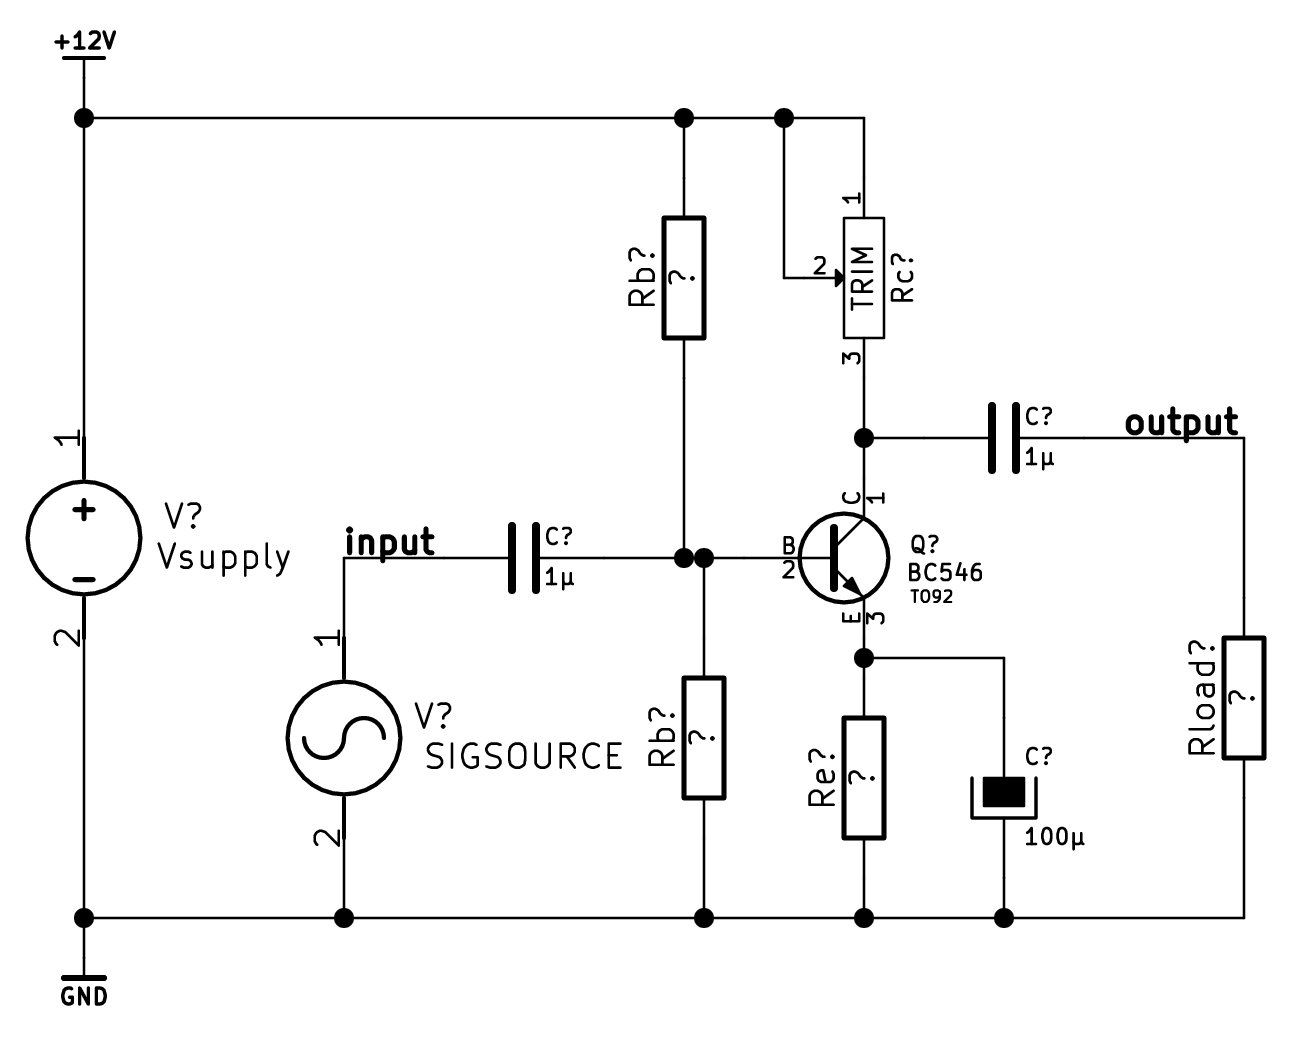
\includegraphics[width=0.75\textwidth]{img/bjt-bias_2AC_improved.png}
    \caption{Voltage divider bias.}
    \label{fig:bjt-bias_2AC_improved}
\end{figure}

\subsubsection{``Noiseless'' biasing}\label{noiseless-biasing}
% ------------------------------------------------------------------------------
For small signals and high input impedance, the biasing can be improved further
in terms of bias voltage "stiffness" and power supply noise rejection. 
The bias voltage is derived from a separate low impedance voltage divider,
heavily filtered and almost a short circuit as far as AC signals are concerned.
The bias voltage is tapped with a higher value resistor which effectively sets
the input impedance of the stage.


\begin{figure}[htbp]
    \centering
    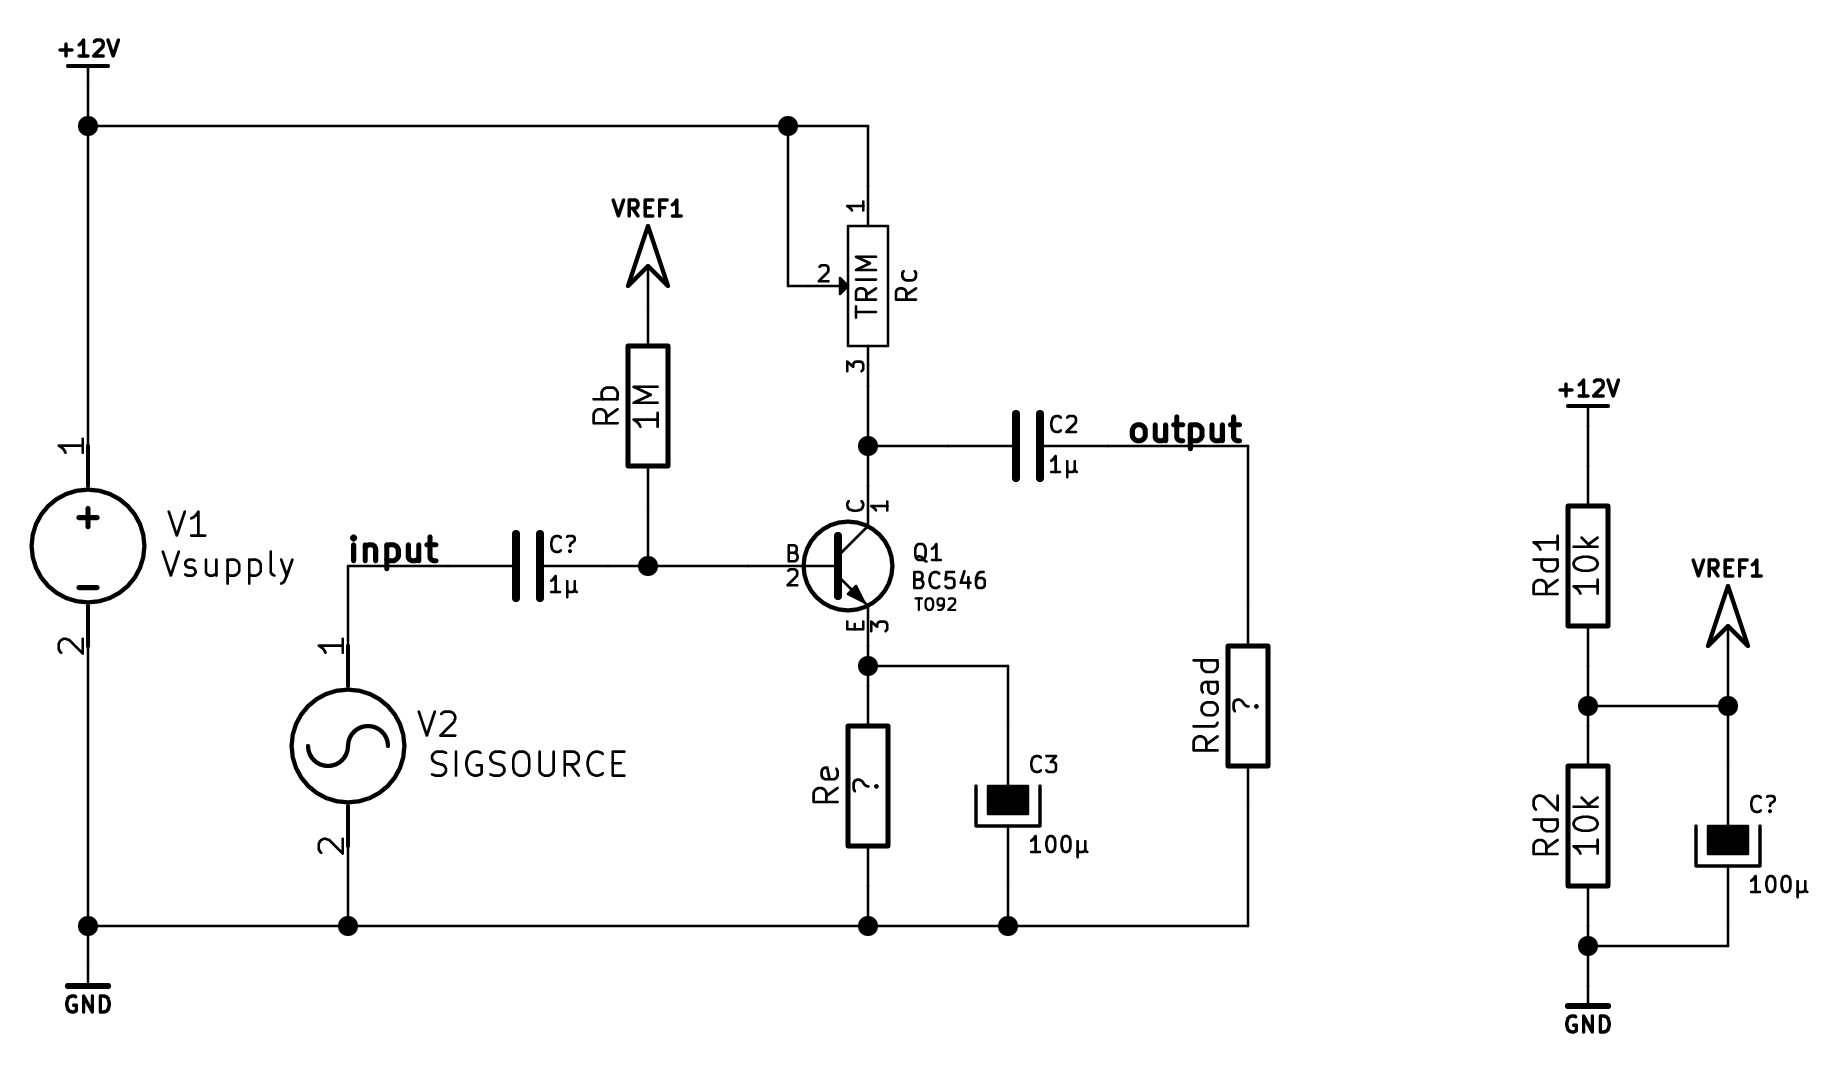
\includegraphics[width=\textwidth]{img/bjt-bias_2AC_quiet.png}
    \caption{Voltage divider with filtered voltage reference.}
    \label{fig:bjt-bias_2AC_quiet}
\end{figure}


\subsection{Comments}\label{comments}
% ------------------------------------------------------------------------------
The AC coupling capacitor forms a high pass filter togeter with the combined
parallel resistance of the biasing network and effective input resistance of
the transistor base. Values of these components is selected to shave off unwanted
frequencies, when dealing with audio often radio frequencies and line voltage hum.
Sometimes you can get away with omitting the input coupling capacitor, but only
if the input signal rides on top of a DC offset. It is considered best practice
to always design circuits for worst case scenarios, I.E. for many scenarios it 
can be beneficial to decouple and current limit all AC signal inputs and outputs.

% ==============================================================================
% SECTION: References
% ==============================================================================
\pagebreak
\section{References}\label{references}

\subsection{www}\label{www}
% ------------------------------------------------------------------------------
Zeghbroech, B. Van - \textit{High injection effects}, accessed 2014-11-28. \\
\url{http://ecee.colorado.edu/~bart/book/book/chapter5/ch5_4.htm}

\subsection{Literature}\label{literature}
% ------------------------------------------------------------------------------

Horowitz P., Hill W. -  \textit{The Art of Electronics}, Cambridge University Press 1989.\\
\medskip 
Horowitz P., Hayes T. - \textit{Student Manual for the Art of Electronics}, Cambridge 1989.

\subsection{Sources}\label{sources}
% ------------------------------------------------------------------------------
Full source, including spice simulation files, CSV data, schematics, etc
is available at \url{https://github.com/jonasjberg/EE413-lab01}


% ==============================================================================
\end{document}
% ==============================================================================